\documentclass{article}
\usepackage[utf8]{inputenc}
\title{Video 1: covariance matrix}
\author{wbg231 }
\date{December 2022}
\newcommand{\R}{$\mathbb{R}$}
\newcommand{\B}{$\beta$}
\newcommand{\A}{$\alpha$}
\newcommand{\D}{\Delta}

\newcommand{\avector}[2]{(#1_2,\ldots,#1_{#2})}
\newcommand{\makedef}[2]{$\textbf{#1}$:#2 }
\usepackage{tikz,graphicx,hyperref,amsmath,amsfonts,amscd,amssymb,bm,cite,epsfig,epsf,url}

\begin{document}

\maketitle

\section{introduction}
\begin{itemize}
\item \href{https://www.youtube.com/watch?v=olyVNcJknNg&ab_channel=CarlosFernandez-Granda}{video link}
\item today we are going to talk about the covariance matrix which captures the variance of multi dimensional features. 
\subsection*{motivation}
\item our goal is to describe data with multiple features 
\item we are going to be working with a random vector $\tilde{x}\in mathbb{R}^{d}$ such that $$\tilde{x}=\begin{pmatrix}
    \Tilde{x}_1\\..\\\Tilde{x}_n
\end{pmatrix}$$
that is each element of the random vector $\tilde{x}$ is it's self a random vector
\section*{mean of random vector}
\item \textbf{the mean of a random vector} $\Tilde{x}\in mathbb{R}^{d}$ is defined as the mean of each of the random vectors
 dimensions that is$$E[\tilde{x}]=\begin{pmatrix}
    E[\Tilde{x}_1]\\..\\E[\Tilde{x}_n]
\end{pmatrix}$$
\subsection*{gaussian random vector}
\item a random vector gaussian random vector $x\in \mathbb{R}^{d}$ has joint pdf $$f_{\tilde{x}}(x)=\frac{1}{\sqrt{(2\pi)^d|\Sigma
|}}e^{-\frac{1}{2}(x-\mu)^t\Sigma^{-1}(x-\mu)}$$
\item where $\mu\in \mathbb{R}^d$ is the mean parameter and $\Sigma\in \mathbb{R}^{d\times d }$ is the covariance matrix 
\item note that what we saw in 1-dimension holds and $E[\Tilde{x}]=\mu$ as we would expect
\item 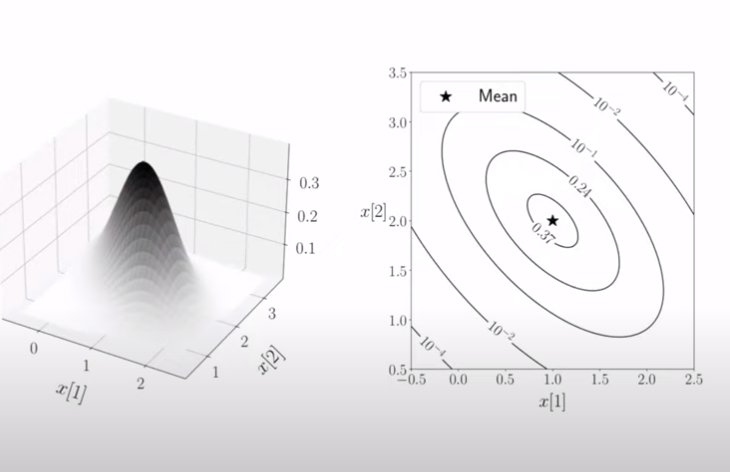
\includegraphics[width=10cm]{/home/buzgalbraith/work/school/spring_2023/probaility-theroy-2-2023/notes/week_8/vedio_1/images/v1_1.png}
\item here are visualizations of the pdf of a gaussian random vector 
\subsection*{sample mean}
\item suppose where have a dataset $\mathcal{D}=\{x_1...x_n\}:x_i\in \mathbb{R}^{d}$
\item the sample is given as $m(x):=\frac{1}{n}\Sigma_{i=1}^{n}x_i$ that is we just take the sample mean of each dimension
\subsection*{faces example}
\item suppose we have a dataset where each observation $x_i\in \mathbb{R}^{4096}$ that is a 64 by 64 image represented as a vector
\item 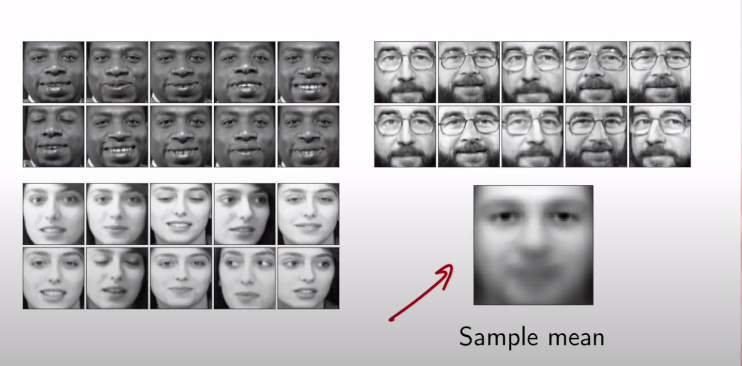
\includegraphics[width=10cm]{/home/buzgalbraith/work/school/spring_2023/probaility-theroy-2-2023/notes/week_8/vedio_1/images/v1_2.png}
\item here the mean is actually meaningfully this is primally because the images are aligned
\subsection*{mean of a random matrix}
\item if we have a random matrix $\Tilde{M}=\begin{pmatrix}
    \Tilde{x}_1& ...& \tilde{x}_{d_2}
\end{pmatrix}\in \mathbb{R}^{d_1\times d_2}:\tilde{x}_i\in \mathbb{R}^{d_1}$ that is a matrix where all columns (or rows) are random vectors and thus all entries are random variables 
\item thus we can see that  $E[\Tilde{M}]=\begin{pmatrix}
    E[\Tilde{x}_1]& ...& E[\tilde{x}_{d_2}]
\end{pmatrix}=\begin{pmatrix}
    E[\tilde{x}_{1,1}] & ... & E[\Tilde{x}]_{1,d_2}\\...&...&...\\E[\tilde{x}_{d_1,1}] & ... & E[\Tilde{x}]_{d_1,d_2}
\end{pmatrix}$
\subsection*{liniarty of expecations}
\item for any random vector $\tilde{x}\in \mathbb{R}^{d}$ deterministic matrix A $\in \mathbb{R}^{n\times d}$ and vector b$\in \mathbb{R}^{n}$
\item what is $E[A\tilde{x}+b]$? 
\item lets look at one entry $E[A\tilde{x}+b][i]$ we know that $(A\Tilde{x}+b)\in \mathbb{R}^{n}$ thus by definition of random vector expectations $E[A\tilde{x}+b][i]=E[\quad [A\tilde{x}+b][i]\quad ]$
\item then we know that $A\tilde{x}[i]$ is a matrix times a vector and thus can be written as $A\tilde{x}[i]=\Sigma_{j=1}^{d}A[i,j]\tilde{x}[j]$ and that will be added onto by the ith entry of b
\item thus we have $E[\quad [A\tilde{x}+b][i]\quad ]=E[\Sigma_{j=1}^{d}A[i,j]\tilde{x}[j]+b[i]]\text{ then we can see that this is an affine } \\\text{  combination of d random varible
  and a constant thus by linearity of expecations} = \Sigma_{j=1}^{d}A[i,j]E[\Tilde{x}_j] +b[i] \text{  and as A is deterministic we can again apply linearity of expectations to get} = (AE[\Tilde{x}]+b)[i]$ 
\item this all more or less goes to show that linearity of expectations holds for random vectors
\item the same thing also holds for random matrix $\tilde{M}\in \mathbb{R}^{n\times d}$ and deterministic matrices $A\in \mathbb{R}^{x \times n}, A\in \mathbb{R}^{x \times d}$ we have $$E[A\Tilde{X}+b]=AE[\Tilde{X}]+B$$
\item this will help us with the covariance matrix 
\section{variance}
\item the variance characterizes the average variation of a random variable
\item for a random vector we can think of the variance as comprised of the linear combination of all entries of the random vector
\subsection*{variance of a linear combination}
\item for any deterministic vector $a$  
\item $var(<a,\Tilde{x}>)=var(a^t\Tilde{x})=E[(a^t\Tilde{x}-E[a^t\Tilde{x}])]=\\
=E[(a^t\Tilde{x}-a^tE[\Tilde{x}])^2] = E[a^t(\tilde{x}-E[\tilde{x}])^2]$
\item here we are going to take a second and define $c_t(\Tilde{x})=\Tilde{x}-E[\Tilde{x}]$ that is the centered version of the random vector  $\Tilde{x}$
\item $var(<a,\Tilde{x}>)=var(a^t\Tilde{x})=E[(a^t\Tilde{x}-E[a^t\Tilde{x}])]=\\
=E[(a^t\Tilde{x}-a^tE[\Tilde{x}])^2] = E[a^t(\tilde{x}-E[\tilde{x}])^2]=E[(a^tc_t(\Tilde{x}))^2]=E[(a^tc_t(\Tilde{x}))(a^tc_t(\Tilde{x}))^{t}]=E[(a^tc_t(\Tilde{x}))(c_t(\Tilde{x})^t a]=a^t E[ct(\Tilde{x}) (ct(\Tilde{x})^t)]a$
\item this is the covariance matrix as we will show 
\item lets take a look at the entries of this matrix $E[ct(\Tilde{x}) (ct(\Tilde{x})^t)[i,j]]$
\item first consider diagonal entries  $E[ct(\Tilde{x}) (ct(\Tilde{x})^t)[i,i]]=E[ct(\Tilde{x}_[i])^2]=E[(\tilde{x}[i]-E[\tilde{x}[i]])^2]=var(\tilde{x}[i])$
\item consider the off diagonal now $E[ct(\Tilde{x}) (ct(\Tilde{x})^t)[i,j]]=E[ct(\Tilde{x}[i]) ct(\tilde{x})[j]]=E[(\Tilde{x}[i]-E[\tilde{x}[i]])*(\Tilde{x}[j]-E[\tilde{x}[j]])]=cov(\Tilde{x}[i],\tilde{x}[j])$
\item so with this in mind we are able to define \textbf{the covariance matrix} of a random vector $\Tilde{x}$ as $$\Sigma_{\tilde{x}}=E[ct(\tilde{x})ct(\tilde{x})^t]=\begin{pmatrix}
    var(\Tilde{x}[1])&cov(\Tilde{x}[1],\tilde{x}[2])&...&...cov(\Tilde{x}[1],\Tilde{x}[d])\\
    cov(\Tilde{x}[1],\Tilde{x}[2])& var(\Tilde{x}[2])&...&cov(\Tilde{x}[2]\Tilde{x}[d])
    \\ cov(\Tilde{x}[i],\tilde{x}[d])&...&... & var(\Tilde{x}[d])
\end{pmatrix}$$
\item the covariance matrix captures the variance of any linear combinations of the random vector
\item so for any deterministic vector $a\in \mathbb{R}^{d}$ $$var[a^t\Tilde{x}]=a^tE[cv(\Tilde{x})cv(\Tilde{x})^t]=a^t\Sigma_{\Tilde{x}}a$$
\item this is nice as this captures the variance of all possible linear combinations
\subsection*{deli example}
\item suppose we have a deli with 3 ingredients bread local cheese and imported cheese
\item suppose that the random vector $\Tilde{x}=\begin{pmatrix}
    \text{price of bread}
    \\ \text{price of local cheese}\\
    \text{ price of imported cheese}
\end{pmatrix}$ 
\item and has covariance matrix $\Sigma_{\tilde{x}}=\begin{pmatrix}
    1&.8&0\\.8&1&0\\0&0&1.2
\end{pmatrix}$
\item this tells us that the price of the bread and local cheese are highly correlated and the price of the imported cheese is uncorrelated
\item there are two recipes we are considering
\item 1. 100 g bread, 50 g local cheese, 50 g imported cheese can be written as vector $a_1\tilde{x}=\begin{pmatrix}
    100\\50\\50
\end{pmatrix}\tilde{x}$ 
\item 2. 100 g bread, 100 g local cheese, 0 g imported cheese can be written as vector $a_2\Tilde{x}=\begin{pmatrix}
    100\\100\\0
\end{pmatrix}\Tilde{x}$ 
\item what is the variance in the price of each recipe?
\item as said before the variance of a linear combination of our random vector can be expressed as $var(a_1\tilde{x})=a_1^{t}\Sigma_{\Tilde{x}}a_1$
\item computing this out we see $a_1$ has lower variance. this makes sense as we are getting a lot of local cheese and bread which are highly correlated so those variances feed off of one another.  
\subsection*{gaussian random vector}
\item a random vector gaussian random vector $x\in \mathbb{R}^{d}$ has joint pdf $$f_{\tilde{x}}(x)=\frac{1}{\sqrt{(2\pi)^d|\Sigma
|}}e^{-\frac{1}{2}(x-\mu)^t\Sigma^{-1}(x-\mu)}$$
\item where $\mu\in \mathbb{R}^d$ is the mean parameter and $\Sigma\in \mathbb{R}^{d\times d }$ is the covariance matrix 
\item note that what we saw in 1-dimension holds and $E[\Tilde{x}]=\mu$ as we would expect
\item we also have $\Sigma_{\Tilde{x}}=\Sigma$
\item 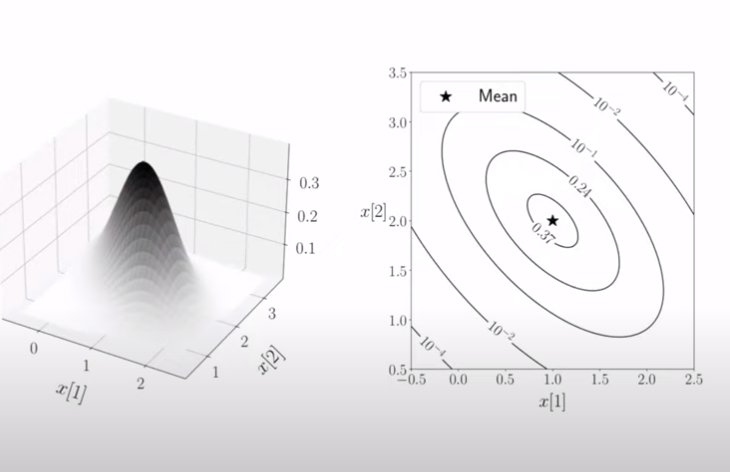
\includegraphics[width=10cm]{/home/buzgalbraith/work/school/spring_2023/probaility-theroy-2-2023/notes/week_8/vedio_1/images/v1_1.png}
\item here are visualizations of the pdf of a gaussian random vector 
\item basically the shape of the ellipsoids for the contour lines are determined by the covariance matrix
\section{variance in a certain direction}
\item if we want to know the variance of a random vector $\Tilde{x}\in \mathbb{R}^{d}$ in a certain direction $b\in \mathbb{R}^{d}$
\item we can think of this  as the variance of  the projection of our random variable onto that direction
\item so if we assume b is unit norm  than $||b||=1$ and $P_{b}(\Tilde{x})=\frac{b^t\Tilde{x}}{||b||}=b^t\Tilde{x}$
\item we are using unit norm directions to make our math easier, and because you can just rescale any vector to be unit norm 
\item further note that $\Tilde{x}=((b^t\Tilde{x}))b+(\Tilde{x}-((b^t\Tilde{x}))b))$ to see this basically notice that $b^t\Tilde{x}$ is the projection of x on to b, and thus $(b^t\Tilde{x})b$ will be collinear (parallel) with b and thus if we subtract that value from our original vector x we are taking away the orthogonal portion of x
\item  here we also assume that we have centered x by subtracting it's mean. 
\item 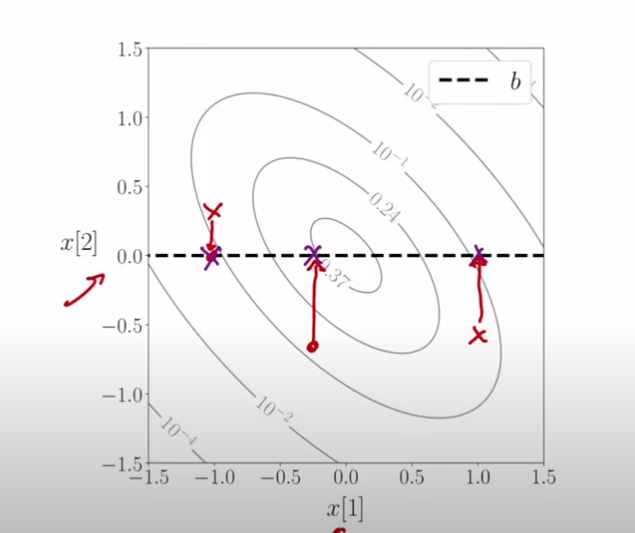
\includegraphics[width=10cm]{/home/buzgalbraith/work/school/spring_2023/probaility-theroy-2-2023/notes/week_8/vedio_1/images/v1_3.png}
\item  here we can see a gaussian rv x, centered at 0 
\item and a direction b
\item then we want to understand how x varies along that line by looking at how much the projection of x $(b^t\tilde{x})$ varies
\item 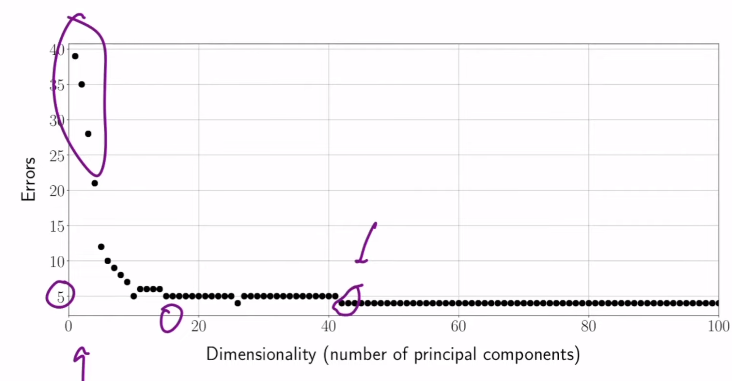
\includegraphics[width=10cm]{/home/buzgalbraith/work/school/spring_2023/probaility-theroy-2-2023/notes/week_8/vedio_1/images/v1_4.png}
\item here is the pdf of $b^t\Tilde{x}$
\item so what is the gaussian from this? we can use our equation $var[b^t\Tilde{X}]=b^t\Sigma_{\Tilde{x}}b=.5$
\item naturally we can do this for any direction
\item 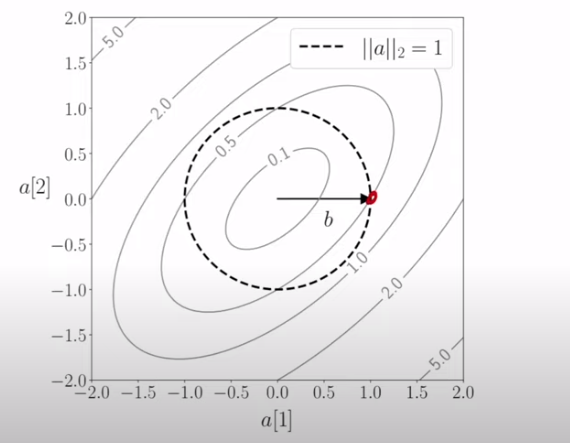
\includegraphics[width=10cm]{/home/buzgalbraith/work/school/spring_2023/probaility-theroy-2-2023/notes/week_8/vedio_1/images/v1_5.png}
\item here is our variance in every direction along the unit circle (ie all vectors with length 1 in $\mathbb{R}^{2}$)
\item 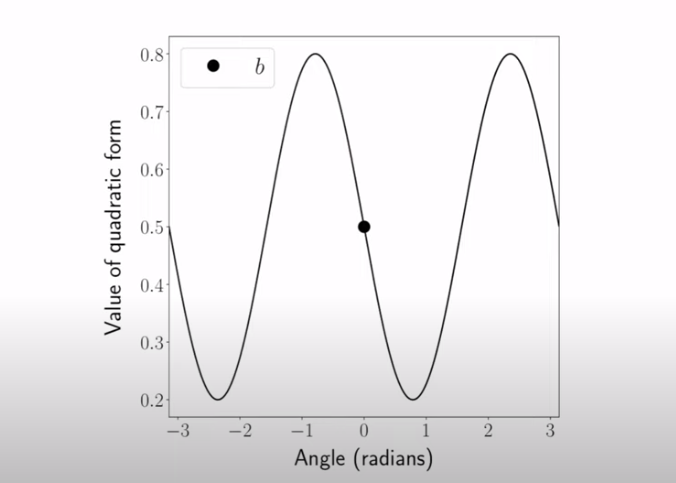
\includegraphics[width=10cm]{/home/buzgalbraith/work/school/spring_2023/probaility-theroy-2-2023/notes/week_8/vedio_1/images/v1_6.png}
\item we can look at this in 1 dimension, and see our variance in a certain direction as a function of the angle (note it is sinusoidal )
\item this is called a quadratic form 
\section*{covariance matrix on a data set}
\item suppose we have dataset $\mathbb{D}=\{x_1...x_n\}\in \mathbb{R}^{d\times n}$
\item we can call the jth feature of our data set $x[j]=\{x_1[j]..x_n[j]\}\in \mathbb{R}^{n}$
\item the sample variance of a feature is  $v(X[j])$
\item and the sample covariance of two features is $c(X[j],X[k])$
\item so here we can deffine the sample covariance matrix as $\Tilde{x}$ as $$\Sigma_{\tilde{x}}=\begin{pmatrix}
    v({x}[1])&c({x}[1],\tilde{x}[2])&...&...c({x}[1],{x}[d])\\
    c({x}[1],{x}[2])& v(\Tilde{x}[2])&...&c(\Tilde{x}[2]\Tilde{x}[d])
    \\ c(\Tilde{x}[i],\tilde{x}[d])&...&... & v(\Tilde{x}[d])
\end{pmatrix}= \frac{1}{n-1}\Sigma_{i=1}^{b}ct(x_i)ct(x_i)^{t}$$ where $ct(x_i)=x_i-m(x)$
\subsection*{sample variance in any direction}
\item $\mathcal{D}=\{x_1..x_n\}$
\item for any vector a $\mathcal{D}_{a}=\{a1^tx_1...a^tx_n\}$
\item then we can find the variance as $var(\mathcal{D}_a)=\frac{1}{n-1}\Sigma_{i=1}^{n}(a^tx_i-\frac{1}{n}\Sigma_{j=1}^{n}a^tx_j)^2$
\item then by doing more or less the same computations as in the random variable case we can see that $var(\mathcal{D}_{a})=a^t \Sigma_{x}a$
\item so the sample covariance matrix also exactly captures the sample variance of any linear combination of the data 
\item so we can do a similar thing as we did in the random case and try to do this along all unit norm vectors to get an idea of the sample variance in all directions as a function of angle


\end{itemize}
\end{document}
